\documentclass[10pt, twocolumn]{article}
\usepackage[utf8]{inputenc}
\usepackage[margin=0.75in]{geometry}
\usepackage{setspace}
\usepackage[pdftex]{graphicx}
\DeclareGraphicsExtensions{.jpg}

\title{\vspace{-2.0cm} Artificial Intelligence Techniques and the "Pronto Pup Problem" }
\author{Christopher Saiko}

\begin{document}
\maketitle

\section{Introduction}

Computer simulations of real world situations are one of the primary areas that we use,
as computer scientists, to describe and model the world around us. By creating and running
these simulations, we may advance our knowledge and ideas about how the real world reacts
to systems that we create. One such large system is the yearly Minnesota State Fair. This
yearly human gathering sees millions of people gather in one place over the course of 10 days.
Summer of 2018 saw an attendance record of over two million people \cite{mnstatefair}, so
it is important to understand how people may move, and how resources may be allocated within
such a system.

One part of such a system is one of the myriad of food stands which are frequented by fair
attendees, and which might also be modeled in such a way as to simulate it. One example, a
Pronto Pup (corn dog) stand, could be implemented using a combination of Producer-Consumer buffers
for the fryers and staff, and a Sleeping Barber implementation \cite{sleepingbarber}
for the queue of fair goers. Other variables, such as ambient temperature, time of day,
acceptable waiting time, and others, could be modeled within the system using probabilistic methods.

Once modeled, various Artificial Intelligence techniques could be applied to this system
to find an allocation of resources to serve a maximum number of customers, while minimizing
the cost to operate the food stand. After creation of such a model, of the techniques used
to solve it, the Hill Climbing algorithm saw the best success at tackling
this so called "Pronto Pup Problem".

\section{Methods}

To determine an efficient allocation of required resources, a number of simulations
needed to be run. To start, a function was developed which may be passed multiple
variables. Within this function, a day of corn dog stand operation was simulated using
the desired parameters and stored variables, and an objective function score returned
at the end. This score is determined by four primary metrics.

Fair attendees served,
a maximized item, represents a total running count of how many customers have been successfully
served food or a beverage. Wasted food items, a minimized item, keeps track of the
amount of wasted product at the end of the business day. Third, the total amount of lost
customers who exited the line queue before being served are tracked. Finally, total
profit, a maximized item, represents the total dollar amount that the
stand generated above operating expenses over the course of a business day.
An algorithm sequentially ran a series of these corn dog stand simulations
to determine the best allocation of resources to the stand. Several Artificial
Intelligence techniques were be used in the algorithm when running the simulation
to determine a best solution.

\section{Algorithms}
\subsection{Corn Dog Stand Simulation}
The simulation algorithm implemented is sequential in nature, to ease implementation
requirements, and to reduce possible varying data collection speeds on multi-core processor systems.
Within the simulation are a possibility of five bounded buffers;
two fryers, two lines for customers, and a general food buffer to place cooked items.
These bounded buffers are be able to be adjusted in size to account for larger or
smaller space allowed. Other variables passed to the algorithm include worker wage rate,
the hours of operation, corn dog and beverage prices, corn dog and beverage costs,
corn dog cook time, daily hourly temperature as an array, number of customer lines, and
acceptable customer wait time. Finally, customer behaviors are passed in the form
of an array, as a series of probabilities between zero and one. Customer arrival
chance per minute is the probability that in any given minute, a customer will arrive,
and be placed into an available line queue.  Corn dog order chance, and corn dog order
chance mealtime offset, respectively, details the probability that a given customer will order a corn dog,
as well as an increase in that chance dependent on the proximity to mealtime,
coded as 8AM, 12PM, 4PM, and 8PM. Beverage order chance, beverage order chance mealtime offset,
and beverage order chance temperature offset, like corn dog order chance, represents
the probability that a given customer will order a beverage, with a similar offset for
proximity to mealtime and an additional chance that the beverage order will be adjusted based on
the current temperature.
\bigbreak
Although some choices for the variables may be arbitrary, real world limits are placed
on the majority of the variables. Fryer number is limited to one or two fryers, and customer
lines are limited to one or two lines. Fryer size capacity is limited to be between
three and six corn dogs, chosen arbitrarily to roughly fit real world fryers. Customer lines size are
not be limited to any particular size, since customers will naturally
grow tired of waiting for service, and leave of their own accord. To ease simulation requirements,
the ambient temperatures have been chosen arbitrarily, as mentioned above. In real world usage
could be decided beforehand by consulting a weather forecast. Customer service time was
fixed at one customer serviced per minute.
\bigbreak
Using all these variables, the algorithm simulates the passage of a single day in
steps of minutes, cooking corn dogs in the fryer queue(s), transferring cooked corn dogs
into a food queue, and placing customers into line queues for service. At the end of the simulated
day, the algorithm calculates profit, wasted food, total customers served, and total customers lost.
These values are used to calculate a score, with varying weights associated with each value.
The simulation is run a total of 1000 times, and returns the average score
for that permutation of variables.

\subsection{Tree Search}
To implement a Tree Search approach to the problem, this algorithm tests
each possible permutation of the variables. Since all variables must be assigned
to have a full state, only the leaves of the resulting tree structure will have possible
solutions, so a Breadth First Search or Depth First Search will be functionally the same.
It is expected that this will not be useful in finding a quality solution, as the number of
variables over which to search is quite large, and time complexity may be too large for a Tree Search to handle. A limit on
the number of simulations is required for Tree Search. Since limiting in this
way may not allow reaching of certain portions of the tree, this method
is to be treated as a lower bound for performance of the simulation. To that end,
a time limit was placed on the algorithm to achieve a possible solution,
and the best scores found and recorded for each time allotment.

\subsection{Hill Climbing}
Local search techniques were then also attempted, specifically Hill Climbing and
Simulated Annealing.\cite{damouth} These algorithms were compared, and their
effectiveness measured, in the context of the score each algorithm achieves. To measure this,
each algorithm recorded the time complexity required, in the form of total
algorithm wall running time, and the best solution found, in the form of the best score value returned from the objective
function. A simple neighbor selection function was be designed, to randomly select
a argument of the simulation algorithm and to randomly shift it to a different valid value.
These neighbors were used to generate a way for the algorithms to choose a new permutation of
variables to simulate.

In the Hill Climbing algorithm, the algorithm selects a neighbor and runs a simulation for
that neighbor. If a better score is found, the new set of variables that resulted in the score
is saved, and a neighbor to that new set of variables is found to test. If a better score is not
found, a new neighbor to the last set of variables to have a better score is found, and tested. This method
is repeated, and as neighbors are found in higher scoring areas of the tree, the algorithm heads in
that direction, climbing the hill to find maximum values.

\subsection{Simulated Annealing}
The Simulated Annealing algorithm, like the Hill Climbing algorithm, utilizes a neighbor function to get
a new set of variables to test. However, unlike Hill Climbing, it may travel further away from an
given state, even with lower resulting scores, attempting to get out of any local maximums which
would otherwise trap the Hill Climbing algorithm. To that end, the algorithm takes three additional values:
alpha, temperature, and end. As the algorithm searches and finds scores among neighbors, it may accept a worse
score with lessening probability as the algorithm proceeds. \cite{codeproject} If a worse
solution is found, instead of rejecting it outright, the algorithm generates a random number
between zero and one, and compares it with exp(-score difference / temperature). If the random
number is higher, the algorithm reject the solution, but if not, it will be accepted.
Every iteration of the algorithm, the temperature is reduced by multiplying the temperature by alpha.
Over time, as the temperature approaches zero, the value of
exp(-score difference / temperature) approaches zero, and the likelihood of worse values being accepted
will be reduced. When the temperature is reduced enough to be below the end value, the
algorithm exits, with the last best value being returned.

\section{Experiments}
In total, three experiments were run, and for each experiment there were a total of sixteen
variables which could be changed within the simulation. The score generated at the end of every set of
a variable set's simulations was calculated as:

\medskip
score = 4 * Dollars Profit + 3 * Served Customers - 2 * Lost Customers - Corn Dogs Wasted
\medskip

The following experiments were run with three different Artificial Intelligence algorithms, with
each being used to select subsequent permutations of corn dog stand variables.

\subsection{Tree Search}
The first experiment, Tree Search, used execution time limits of 60 seconds, 120 seconds, and
600 seconds. Each time the simulation was run with a set of variables, it was repeated 1000
times to reduce possible effects from the randomness in customer behaviors. Each run time
was performed five times, the resulting score recorded, and the variables used for the high
score simulation recorded.

\subsection{Hill Climbing}
The second experiment, Hill Climbing, used execution time limits again of 60 seconds, 120 seconds,
and 600 seconds. Like Tree Search before, each time the simulation was run with a set of variables,
it was repeated 1000 times to reduce possible effects from the randomness in customer behaviors. Each
timed run was performed five times, the resulting score recorded, and again, the variables used
for the high score simulation recorded.

\subsection{Simulated Annealing}
Finally, the third experiment utilized Simulated Annealing. Unlike the previous
two algorithms, Simulated Annealing operated by starting with variables of alpha,
temperature, end, and number of iterations. Default initial values of alpha = 0.98,
temperature = 1000, end = 0.01, and iterations = 50000 were first used to run
the algorithm five times. Then, the temperature was increased to 10000, with the
other values held at default, and the algorithm again run five times. Subsequent
sets of runs were then carried out with temperature values of 20000 and 100000.

Returning to all default values, alpha was set to 0.95, with the other values still
kept at default, and the algorithm run five times. A further two sets of runs were
performed with alpha set to 0.9 and 0.85, with the default values for other settings.
With each set of runs, the best score found using the algorithm was recorded,
the wall time required to run, as well as the variables used to get that score. As with the previous
two experiments, each set of simulation variables to be simulated was repeated 1000 times
and the score averaged.

\section{Results}
\subsection{Tree Search}
The first experiment, regarding Tree Search, gave expected results. Due to the enormous
number of potential permutations of the variables, the Tree Search in all cases never
managed to get through the majority of the tree. Despite this, it can be seen that as the algorithm
is allowed to run for a longer time, higher scores are found, as more of the tree is explored. The 20 second
Tree Search was found to have a mean score of 5135.6 and a standard deviation of 10.35. The 120 second Tree Search
was found to have a mean of 6405.2 and a standard deviation of 289.07. Finally, the 600 second
Tree Search had a mean score of 7629.6 and a standard deviation of 8.438. Table 1 shows
the raw data from the different runs. Figure 1 shows the
variation between the different run times selected for this experiment.

\bigbreak
\begin{tabular}{ |p{1.3cm}||p{1.3cm}|p{1.3cm}|p{1.3cm}|  }
 \hline
 \multicolumn{4}{|c|}{Table 1: Tree Search Data} \\
 \hline
     &20 sec&120 sec&600 sec\\
 \hline
  Run No. & Score & Score & Score\\
 \hline
   1 & 5127 & 6681 & 7635\\
   2 & 5141 & 6053 & 7633\\
   3 & 5137 & 6056 & 7627\\
   4 & 5136 & 6567 & 7628\\
   5 & 5137 & 6669 & 7625\\
 \hline
 Mean & 5135.6 & 6405.2 & 7629.6\\
 \hline
 Std Dev& 4.63 & 289.07 & 3.77\\
 \hline
\end{tabular}
\bigbreak


As seen from the data, the standard deviation for the Tree Search experiment is overall lower
when compared to the other data. This is to be expected, since the algorithm, when limited by wall time
in execution, will end up at roughly the same point in the state space as the algorithm
traverses the tree, and it would be expected that the same set of variables should produce very similar
results at the same place within the tree. That the score increases with time is also expected. As the
algorithm is allowed more time to execute, it has the opportunity to explore more areas of the tree, and so
find sets of variables which will produce a higher score.


\medskip
\begin{figure}[!ht]
\centering
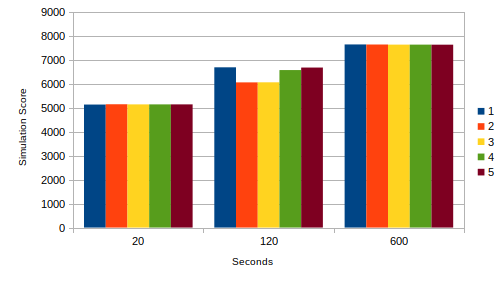
\includegraphics[width=3.6in]{search_scores.png}
\caption{Tree Search Runs and Scores}
\label{fig_1}
\end{figure}
\medskip


Although the scores recorded for this experiment did score lower than the others,
it must be stated that the ordering of the variable selection in the algorithm has
a great effect on the potential scores recorded. It is possible that with a different
ordering, the algorithm could travel to a different section of the tree in the time allowed,
where scores could potentially be higher, or even lower.

\subsection{Hill Climbing}
The second experiment was run using the Hill Climbing algorithm. As expected, this algorithm
generated better results than the preceding Tree Search algorithm, since it may randomly encounter
areas of the tree which will generate a higher resulting score, and then travel deeper into areas
which produce higher scores. The 20 second Hill Climbing algorithm resulted in a mean score of 24738,
and a standard deviation of 7632.7. The 120 second Hill Climbing algorithm had a mean
score of 36017.8 and a standard deviation of 1124.57. Lastly, the 600 second Hill Climbing algorithm
had a mean score of 36456.8 and a standard deviation of 1380.68. Figure 2 shows the variation found between
the different run times for Hill Climbing.

\bigbreak
\begin{tabular}{ |p{1.3cm}||p{1.3cm}|p{1.3cm}|p{1.3cm}|  }
 \hline
 \multicolumn{4}{|c|}{Table 2: Hill Climbing Data} \\
 \hline
     &20 sec&120 sec&600 sec\\
 \hline
  Run No. & Score & Score & Score\\
 \hline
   1 & 24268 & 35401 & 37269\\
   2 & 18524 & 37253 & 37282\\
   3 & 26650 & 37253 & 37262\\
   4 & 25556 & 34325 & 36711\\
   5 & 28692 & 35857 & 33760\\
 \hline
 Mean & 24738 & 36017.8 & 36456.8\\
 \hline
 Std Dev& 3429.10 & 1124.57 & 1365.75\\
 \hline
\end{tabular}
\bigbreak

As detailed in the data above, it appears that the additional time afforded to the Hill
Climbing algorithm in the 600 second runs had a much smaller effect compared to the other two
runs than there was in the case of the Tree Search algorithm. It is expected that
an increase in allowable running time would produce a better score, since the Hill Climbing
algorithm will have more time to reach the maximum of any scores found within the tree.
Of all the AI algorithms attempted in these experiments, Hill Climbing
saw the best result in the form of highest scores.

\medskip
\begin{figure}[!ht]
\centering
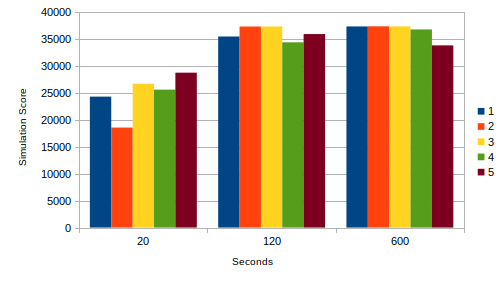
\includegraphics[width=3.5in]{climbing_scores.png}
\caption{Hill Climbing Runs and Scores}
\label{fig_2}
\end{figure}
\medskip

As seen in Figure 2, scores found for runs in the Hill Climbing experiment appear to
level off around the 120 second runs of the experiment. Although the 600 second runs have
an average score that is just over 1.2\% higher than the 120 second runs, the 120 second runs
have a standard deviation that is 17.7\% lower than the 600 second runs. This indicates
that the 120 second run of the Hill Climbing algorithm has the better quality in finding
a closer, more accurate simulation score.

\subsection{Simulated Annealing}
The third and final experiment was carried out using the Simulated Annealing algorithm.
Performance in all cases for this technique was found to be less than that of Hill Climbing.
The two changed variables within the Simulated Annealing algorithm were the initial
temperature selected, and the initial alpha selected. For the Simulated Annealing
temperature runs, the 1000 temperature run had a mean score value of 25623.6 and
a standard deviation of 1954.73. The 10000 temperature run had a mean score value
of 26009.6 and a standard deviation of 1250.54. The 20000 temperature run had a
mean score value of 26233.4 and a standard deviation of 1604.76. Finally, the
100000 temperature run had a mean score value of 25426.4 and a standard deviation
of 2484.03.

\bigbreak
\begin{tabular}{ |p{1.3cm}||p{1.2cm}|p{1.2cm}|p{1.2cm}|p{1.2cm}|  }
 \hline
 \multicolumn{5}{|c|}{Table 3: Simulated Annealing: Temperature Data} \\
 \hline
     & 1000 & 10000 & 20000 & 100000\\
 \hline
  Run No. & Score & Score & Score & Score\\
 \hline
   1 & 24881 &	26836 &	27682 &	30188\\
   2 & 28233 &	23714	& 26452	& 24607\\
   3 & 22374 &	25669	& 24333	& 25258\\
   4 & 25977 &	26677	& 24467	& 23963\\
   5 & 26653 &	27152	& 28233	& 23116\\
 \hline
 Mean & 25623.6	& 26009.6&	26233.4&	25426.4\\
 \hline
 Std Dev& 1954.73 &	1250.54 &	1604.76 &	2484.03\\
 \hline
\end{tabular}
\bigbreak

As shown by the data in Table 3 and Figure 3, increasing the initial temperature did not have
a discernible effect on the mean score found between the runs, and may not be useful in finding
better scores. Only the Simulated Annealing 10000 temperature run had a standard
deviation close to the two high scoring Hill Climbing runs. Even the 20 second Hill Climbing
run only barely lost in scoring to every Simulated Annealing Temperature run, though all have a better
standard deviation than that particular Hill Climbing run.

\medskip
\begin{figure}[!ht]
\centering
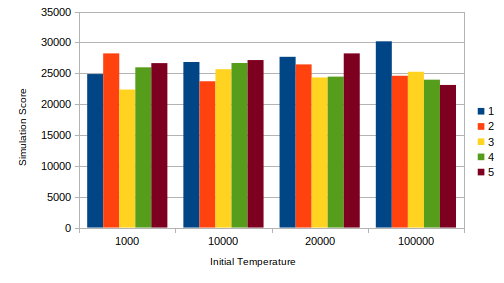
\includegraphics[width=3.5in]{temperature_scores.png}
\caption{Simulated Annealing Temperature Runs and Scores}
\label{fig_3}
\end{figure}
\medskip

For the Simulated Annealing Alpha runs, the 0.98 alpha run had a mean score value of 25623.6 and
a standard deviation of 1954.73. The 0.95 alpha run had a mean score value
of 24185 and a standard deviation of 2837.83. The 0.9 alpha run had a
mean score value of 22213.8 and a standard deviation of 5863.50. Finally, the
0.85 alpha run had a mean score value of 18205.2 and a standard deviation
of 6487.23.

\medskip
\begin{figure}[!ht]
\centering
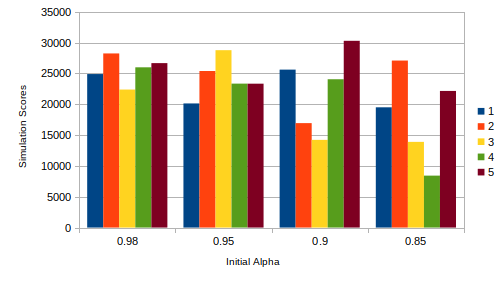
\includegraphics[width=3.5in]{alpha_scores.png}
\caption{Simulated Annealing Alpha Runs and Scores}
\label{fig_4}
\end{figure}
\medskip

Figure 4 and Table 4 show the data collected from the Simulated Annealing Alpha runs. As the
value of alpha is lowered, even by these initial small amounts, the resulting scores
quickly become erratic, as seen in Figure 4. Table 4 also shows how the standard deviation
grows as the alpha value drops, as well as demonstrating the mean score drop as the alpha value drops.
This is expected, since by lowering the value of alpha, the number of iterations over which the algorithm
has to run the algorithm drops, through the temperature cooling much faster. Since the number of
iterations is lower, the number of variable states encountered is lower, and higher scores may not be
encountered.

\bigbreak
\begin{tabular}{ |p{1.3cm}||p{1.2cm}|p{1.2cm}|p{1.2cm}|p{1.2cm}|  }
 \hline
 \multicolumn{5}{|c|}{Table 4: Simulated Annealing: Alpha Data} \\
 \hline
     & 0.98 & 0.95 & 0.9 & 0.85\\
 \hline
  Run No. & Score & Score & Score & Score\\
 \hline
   1 & 24881 &	20125	& 25602	& 19491\\
   2 & 28233 &	25384	& 16929	& 27078\\
   3 & 22374 &	28755 &	14211	& 13887\\
   4 & 25977 &	23334	& 24045	& 8417\\
   5 & 26653 &	23327	& 30282	& 22153\\
 \hline
 Mean & 25623.6	& 24185	& 22213.8	& 18205.2\\
 \hline
 Std Dev& 1954.73&	2837.83&	5863.50&	6487.23\\
 \hline
\end{tabular}
\bigbreak

\subsection{Run Time}
One final comparison to be made between the algorithms is that of their running time. While
the Tree Search and Hill Climbing are limited in their running time by design, Simulated
Annealing only ends when temperature within the algorithm has cooled enough that the algorithm
exits. Although the iterations are constant among runs of each Simulated Annealing type, additional
algorithm work may affect the total run time. Figure 5 shows a comparison between the best scoring, lowest
standard deviation runs of Hill Climbing and Simulated Annealing, and their mean run time to
complete.

\medskip
\begin{figure}[!ht]
\centering
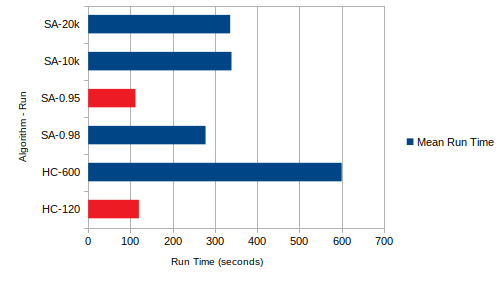
\includegraphics[width=3.5in]{runtime_compare.png}
\caption{Algorithm Runtime Comparisons}
\label{fig_5}
\end{figure}
\medskip

As shown, only the Simulated Annealing 0.95 Alpha runs do marginally better than the Hill Climbing 120 second
runs (highlighted in red). Figure 6 shows the mean scores for the same experiment runs
as Figure 5, with the same two highlighted in red. The Hill Climbing 120 second run has
a vastly better score than the Simulated Annealing 0.95 Alpha run, with only a
small deficiency in mean run time.

\medskip
\begin{figure}[!ht]
\centering
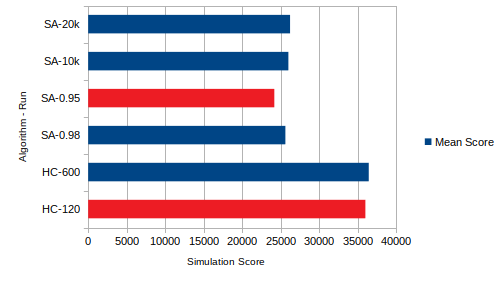
\includegraphics[width=3.5in]{score_compare.png}
\caption{Algorithm Runtime Comparisons}
\label{fig_6}
\end{figure}
\medskip

\section{Conclusion}

The ultimate goal of this research was to determine, among three AI algorithm
techniques, which of them might have the best success at determining the best setup
for a corn dog stand. While the simulation itself was somewhat arbitrary, as a concept
it has value for understanding and modeling human-driven systems, as well as predicting
the behavior of those systems in the real world using Artificial Intelligence.

In the course of these experiments, it was determined that between the algorithms of
Tree Search, Hill Climbing, and Simulated Annealing, Hill Climbing had the best objective performance.
The 120 second runs of the Hill Climbing algorithm had close to the top score, being only
1.2\% behind the 600 second runs of Hill Climbing. Additionally, of the higher scoring runs,
the 120 second runs had the lowest standard deviation, being 17.7\% lower than the 600 second Hill Climbing
runs, and indicating the most accurate scores.
As well, comparing the total run times for the algorithms, Hill Climbing is again superior to
Simulated Annealing and Tree Search. In nearly every run of the experiments, Hill Climbing was found
to have the lowest running time with the highest scores, giving it an efficiency
advantage over Simulated Annealing and Tree Search. Only the Simulated Annealing 0.95 Alpha runs
were in any way comparable in run time, while still having acceptable accuracy.

While a determination was able to be made for which algorithm was useful for finding
the highest, most accurate score within the context of this simulation, it is possible
that with a more complicated simulation algorithm, or more human behaviors, that Hill Climbing
may no longer be the clear choice. Parts of the simulation could be adjusted to be not
permutable, if human behaviors may be observed and narrowed in their probability.
As well, wages paid, as a variable, has no real effect within the simulation other
than to be a range, so of course lower wages will result in
higher profit, and a thus higher score. These are just two examples, and there are
potentially hundreds of other improvements to be made to the Corn Dog Stand Simulation
algorithm, which may have a far reaching effect on what AI algorithms
may be used. However, it appears that Hill Climbing is a good place to start.

\begin{thebibliography}{1}

\bibitem{mnstatefair} https://www.mnstatefair.org/about-the-fair/attendance/. {\em Online, mnstatefair.org}

\bibitem{sleepingbarber} Dijkstra, E.W. ``Cooperating sequential processes,'' {\em Technical Report EWD-123}, Eindhoven University of Technology, The Netherlands, 1965.

\bibitem{damouth} Damouth, Daniel E. and Durfee, Edmund H. ``Local search in the coordination of intelligent agents,'' {\em Proceedings of the National Conference on Artificial Intelligence}, vol. 2, pp. 1437-1437, 1994.

\bibitem{codeproject} https://www.codeproject.com/Articles/13789/Simulated-Annealing-Example-in-C. {\em Online, codeproject.com}

\end{thebibliography}
\end{document}
